\subsection{Определяне на позиция в 3 измерения с помоща на трилатерация и приблизителни разстояния}

В документ \cite{murphy} е разработена система за следене на товарите в 3 измерения в мина чрез използване на трансмитери и получатели [фиг. \ref{fig:mine}]. Използвани са радио трансмитери. Разработен е специализиран лазер, който изчислява височината на товара, без който проблема за 3 измерения се е считал за нерешим. Проблем представляват разликите във височината и останалите измерения тъй като останалите измерения са в пъти по-големи в повечето случаи, както се вижда във фигура \ref{fig:initPos}, тъй като това тази разлика често води до изродени матрици.

\begin{figure}
    \centering
    \centerline{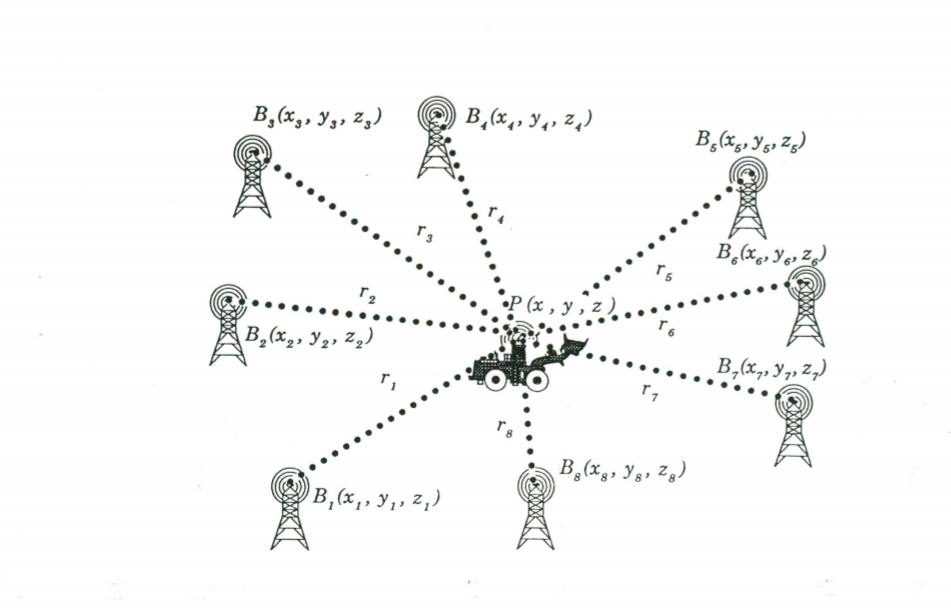
\includegraphics{dt1}}
    \caption{Разположение на получателите и предавателя в мина}
    \label{fig:mine}
\end{figure}

\begin{figure}
    \centering
    \centerline{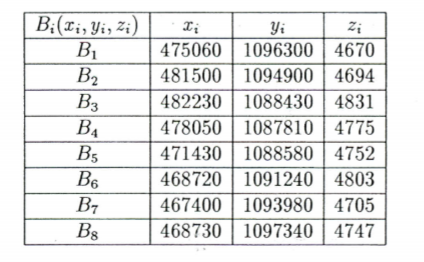
\includegraphics{MurphyInitialPositions}}
    \caption{Начално разположение на статичните получатели}
    \label{fig:initPos}
\end{figure}


\begin{equation}\label{circleEq}
    (x-x_i)^2 + (y-y_i)^2 +(z-z_i)^2=r_i^2
\end{equation}

Разглежда се възможността за съствяне система от \textit{N} на брой нелинейни уравнения използвайки формулата за сфера (уравнение \ref{circleEq}). Задачата се моделира като търсене на пресечни точки на N на брой сфери за всеки трансмитер.

Решението на гореспоменатата нелинейна система от уравнения \emph{се счита за неоптимално} тъй като полученото уравнение е нелинейно и е от висока степен. Когато разстоянията, които са измерени са точни, а не са приблизителни, линезирането на системата от уравнения е удачно. В този случай задачата се преобразува в търсенето на пресечната точка на няколко равнини. Системи с по-малко от тази бройка приемници се считат за неизползваеми. \\

Разглежда се метод за линеризация на уравненията, за който всяка измерена дистанция между трансмитер и получател се използва уравнението за сфера ( кръг в 2D ) ( уравнение \ref{circleEq} ). Методът за линеризация съвпада с този използван в секция \ref{squares_algorithm}. Тъй като има (n-1) уравнения, за долна граница се считат 4 бр. приемника.
\\

Разглеждат се няколко метода за работа с приблизителни разстояния

\begin{itemize}
    \item \strong{Линейни най-малки квадрати} \\ Този метод предоставя по-задоволителни резултати в сравнение с решаване на проблема чрез решение на задачата с линеризиране на уравненията, но не дава оптимални резултати, защото резултатите определят координатите с  грешка повече от 5 фута, което в ситуацията описана в статия \cite{murphy}, е недостатъчно като точност. Тъй като разстоянията са приблизителни се решава уравнение \ref{matrixeq}. Чрез минимизиране на сумата на квадратите на остатъците, уравнение \ref{nonNormalEq} води до уравнение \ref{normalEq}. \textit{[Noble and Daniel 1988]}
    
    \begin{equation} \label{matrixeq}
      A \vec{x} \approx \vec{b} 
    \end{equation}
    
    \begin{equation} \label{nonNormalEq}
        S = \vec{r}^T \vec{r} = (\vec{b} - A \vec{x})^T ( \vec{b} - A \vec{x})
    \end{equation}
    
    \begin{equation} \label{normalEq}
        A^T A \vec{x} = A^T \vec{b}
    \end{equation}
    
        
    Ако матрицата A в изразa $A^T A$ на уравнение \ref{normalEq} не е изродена се използва уравнение \ref{nonSing} , за да се намери решение на задачата.

    \begin{equation} \label{nonSing}
        \vec{x} = (A^T A)^{-1} A^T \vec{b}
    \end{equation}
    
    \item \strong{Нелинейни най-малки квадрати}
    
\end{itemize}


\strong{Резултати}

\begin{figure}
    \centering
    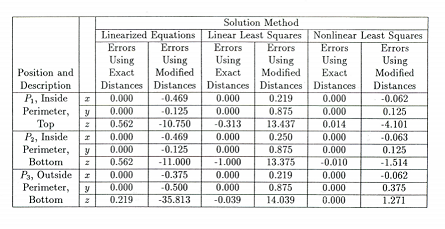
\includegraphics{murphyresults}
    \caption{Резултати при използване на различни методи за изчисление}
    \label{fig:murphyResults}
\end{figure}



Фигура \ref{fig:murphyResults} демонстрира резултатите при определянето на координатите. Най-добри резултати се получават при използването на нелинейни най-малки квадрати, а най-лоши при използването на линеризирани уравнения. Линейните най-малки квадрати водят до най-добри резултати, когато не съществува голяма разлика в стойностите на измеренията (x,y,z).